
\documentclass[preprint,12pt]{elsarticle}

\usepackage[spanish]{babel}
\usepackage{amssymb}
\usepackage{graphicx}
\usepackage{lineno}
\usepackage[utf8]{inputenc}
\usepackage{url}

\journal{Inteligencia de Negocios}

\begin{document}
	
	\begin{frontmatter}
		
		
		\title{\huge Data Story Telling}
		
		\author{Balaguer Valles, Angela Lessly               (2016054494)}
		\author{Huallpa Castro, Leydi Katherine	      (2015053230)}
		\author{Pilco Quispe, Mireya Flavia		      (2015053234)}
		\author{Salamanca Contreras, Fiorella Rosmery (2015053237)}
		
		\address{Tacna, Perú}
		
		\begin{abstract}
			%% Text of abstract
			In this article an analysis is made of why Data Storytelling, or the stories we tell from the analysis of information, is important to make a program of analysis successful.

When talking to people who are successful in the subject of information analytics, usually, at some point, the phrase "tell a story with information" is mentioned. It seems obvious that no one doing a data analysis would like to create a narrative of the process and its results, but for many information analysts, this is not entirely obvious. So this article will explain the reasons why we believe that the information, and the stories created from the analysis of it, are so important.
	
		\end{abstract}
\end{frontmatter}
%%
	%% Start line numbering here if you want
	%%
	%\linenumbers
	
	%% main text
	\section{Resumen}
		En este artículo se hace un análisis de por qué el Data Storytelling, o las historias que contamos a partir del análisis de información, es importante para hacer que un programa de análisis sea exitoso. 

Cuando se habla con personas que tienen éxito en el tema de la analítica de la información, usualmente, en algún punto, se mencione la frase "contar una historia con la información". Pareciera obvio que nadie que esté haciendo un análisis de datos quisiera crear una narrativa del proceso y sus resultados, pero para muchos analistas de información, esto no es del todo obvio. Así que en este artículo se explicarán las razones por las cuales creemos que la información, y la historias creadas a partir del análisis de la misma, son tan importantes.\\

	%%
	%% Start line numbering here if you want
	%%
	%\linenumbers
	
	%% main text

\section{Objetivos}
		\begin{itemize}
		\item Objetivo 1: El objetivo central en este articulo es sintetizar y analizar la importancia que tiene contar historias o relatos en las organizaciones (Storytelling), como una forma de difundir y asimilar los valores, las costumbres y las creencias empresariales.
		\item Objetivo 2: Dar a conocer cuales son los elementos claves y la combinaciones de estos elementos, que beneficios podemos obtener de cada uno de ellos y si es necesario todos los elementos para obtener buenos resultados.
		\item Objetivo 3: Dar ejemplo  como referencia del uso de DataStoryTelling en el mercado y las empresas, logrando destacar los objetivos y beneficios que traen para las mismas.
	\end{itemize}

	%%
	%% Start line numbering here if you want
	%%
	%\linenumbers
	
	%% main text

\section{Marco Teorico}
	\label{S:1}
\subsection{Data Storytelling}	

	El Data Storytelling es una herramienta que emplea la combinación de datos estadísticos y comunicación. Ayuda a las empresas a cumplir metas de comunicación y marketing contando mensajes de manera efectiva y cargados de información relevante para el público objetivo, también apoyados en instrumentos visuales y narrativos.\\
		
	\subsection{Elementos clave}
	
	El llamado Data Storytelling no es más que un enfoque estructurado sobre cómo comunicamos insights a partir de los datos, e involucra una combinación de tres elementos: datos, visualización y narrativa.
Ahora, ¿qué resulta de la combinación de estos elementos?, ¿cómo nos podemos beneficiar de ellos?, ¿necesitamos todos los elementos en cada análisis que hagamos?\\

			\begin{figure}[htb]
				\begin{center}
					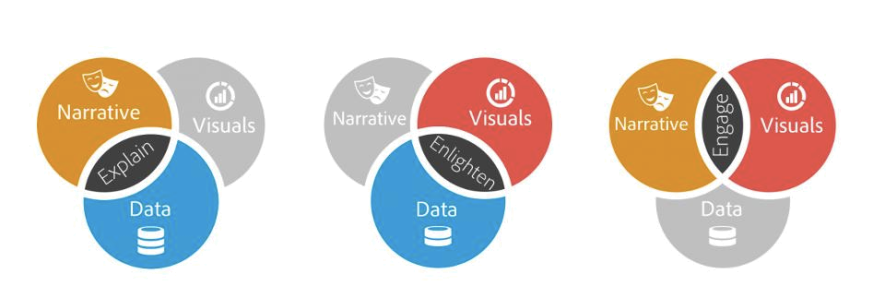
\includegraphics[width=13cm]{./Imagenes/img1}
				\end{center}
			\end{figure}
\begin{itemize}
		\item Narrativa + Datos = podremos explicar qué ha pasado y por qué un insight puede ser importante. Necesitaremos contexto para entender las 	conclusiones por completo.
		\item Visualización + Datos = Enlighten. Cuando añadimos una visualización a nuestros datos, podemos iluminar a nuestra audiencia con insights que no habrían visto de otra manera.
		\item Narrativa + Visualización = Engagement. La combinación perfecta para lograr ese interés e incluso para entretener a nuestra audiencia. 
	\end{itemize}

Pero, cuando unimos Visualización + Narración + Datos = Change, logramos contar una historia con nuestros datos, logramos influenciar y llevar a ese cambio que estábamos buscando.
\begin{figure}[htb]
				\begin{center}
					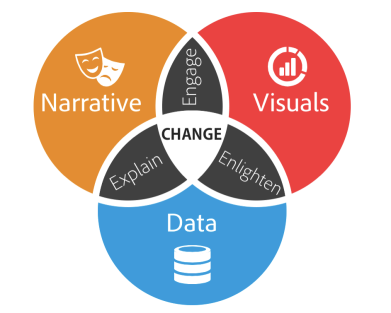
\includegraphics[width=5cm]{./Imagenes/img2}
				\end{center}
			\end{figure}
Y es que la pasión por los datos, ¡tiene que ir acompañada también por la pasión de contar historias! Si comunicas pobremente tus insights o si llegas a conclusiones erróneas, puede ser prácticamente peor que no utilizar ningún dato.

	\textbf{¿Por qué Data Storytelling?}

	\begin{itemize}
		\item Las historias son herramientas efectivas para transmitir la experiencia humana: esto ha sido así desde el inicio de los tiempos, pero ahora utilizamos datos y análisis para crear versiones mejoradas de esas historias. Gracias a ellas simplificamos y damos sentido a un mundo complejo.
		\item Para inspirar el cambio, necesitamos que entiendan nuestra historia: no importa cuántas horas hay detrás de nuestro análisis, no lograremos nada si no nos logramos explicar ya sea con una narrativa o con gráficos pero, necesitamos una historia.

		\item Las personas quieren evidencia del análisis que hay detrás: aunque nuestra audiencia no entienda el detalle de la analítica, sí quieren la evidencia de que hay datos detrás, ya que estas historias son más convincentes que solo una experiencia personal.

		\item Contar en una breve historia el resultado de horas de trabajo: se necesitan presentaciones cortas, con ideas concretas adaptadas a los stakeholders que recibirán la información para hacer llegar tu mensaje de una manera simple. 	
	\end{itemize}

	\subsection{Data Visualization}

	Es muy común que Data Storytelling se entienda solo como visualización de datos y, aunque como estamos viendo, es mucho más que eso, es cierto que la visualización es una parte esencial y muy potente como complementaria al análisis, para poder condensar grandes conjuntos de datos en una sola foto.\\

\subsection{Pero, ¿qué nos permite?}
	
	\begin{itemize}
		\item Comprensión rápida de la información: gracias a las representaciones gráficas podemos ver grandes cantidades de datos de forma clara y coherente, lo que facilita la extracción de conclusiones e insights. Ganaremos tiempo y eficiencia para solucionar problemas.

		\item Identificar y actuar rápido sobre tendencias emergentes: incluso los archivos de datos casi infinitos, empiezan a tener sentido al representarse gráficamente; lo que nos permite detectar parámetros que están altamente correlacionados. Algunas relaciones serán obvias, pero otras tendremos que identificarlas para ayudar al cliente a enfocarse en ese punto de mejora que influenciará en sus objetivos principales.

		\item Identificar relaciones y patrones dentro de los activos digitales: descubrir tendencias dentro de los datos nos puede dar ventaja competitiva, como detectar puntos clave que están afectando a la calidad del producto o solucionar incidencias antes de que se conviertan en mayores problemas.

		\item Desarrollar un nuevo lenguaje de negocio para contar la historia a otros: una vez que hemos descubierto nuevos insights gracias a la analítica visual, el siguiente paso es comunicarlos, ya sea con gráficos simples o visualizaciones elaboradas, pero lo importante es lograr ese engagement y transmitir el mensaje rápidamente.	
	\end{itemize}
Para algunos, el esfuerzo de crear una historia alrededor de sus insights lo consideran innecesario y, además, una pérdida de tiempo. Pero creer que los datos deberían ser suficientes en sí mismos, solo porque sean explicados de una manera sencilla y concisa, para llevar a sus audiencias a tomar las decisiones necesarias, es lo mismo que creer erróneamente que las decisiones de negocio se toman teniendo en cuenta solo la lógica y la razón.\\


	
	El análisis de negocios depende de volúmenes suficientes de datos de alta calidad. La dificultad para garantizar la calidad de los datos es la integración y conciliación de los datos en diferentes sistemas, y luego decidir qué subconjuntos de datos estarán disponibles. \\
\subsection{Para que sirve la data?}

	En ocasiones anteriores, ya habíamos platicado sobre la importancia de las historias en la decisión de compra, de cómo todo lo que nos rodea es narrativa y de por qué la emoción es infalible para llevar a la acción.

En esta ocasión, veremos cuáles son las ventajas de usar data storytelling para tu marca
	\begin{itemize}
		\item Provee valor y significado
Recuerda que la gente usa los buenos contenidos para resolver sus problemas, aprender y lidiar de mejor forma con el mundo. Es por ello que tú como marca deberías saber cómo comunicar tus insights para dotarlos de contexto, de valor y de significado, lo cual, a su vez, otorgará estos mismos valores a tu marca ante los ojos de tu consumidor.

		\item Crea materiales invaluables para relaciones públicas
Aprovecha los datos internos de tu marca para crear historias valiosas que ninguno de tus competidores tendrá. Además, recuerda que los medios siempre están sedientos de historias originales que les den “rating”, visitas, clicks, likes, etc.

		\item La hace creíble
Vivimos saturados de fake news, datos, infografías, presentaciones de PowerPoint y tablas de Excel, y sin embargo, la gente sigue prefiriendo los datos duros para dar credibilidad a lo que está consumiendo. Si tú le das color y vida a esos datos duros mediante una historia interesante, el público será más propenso a creer en los datos que le presentas y te preferirá sobre tus competidores.

		\item Fija tu mensaje en la mente de tu audiencia
La combinación de datos y narrativa permite que tu público aumente su comprensión, retención y su atracción hacia tu marca.

		\item Se hace sexy
Cuando usas storytelling efectivo, lo más probable es que tus audiencias queden “enamoradas” de tu marca sin saber exactamente por qué, y tú, mientras tanto, les comunicas tus mensajes clave, los cuales ellas aceptarán gustosas.

		\item La hace versátil
Gracias a que las historias se pueden presentar de muchas maneras, va a ser difícil que aburras a tus audiencias: puedes usar videos, gifs, artículos, podcast, ebooks, y muchos otros formatos más.
\end{itemize}
 

	%%
	%% Start line numbering here if you want
	%%
	%\linenumbers
	
	%% main text

\section{Ejemplo}
	\label{S:1}

Cualquier gran historia significa visualización y detalle. Se necesitan las pequeñas adiciones de esos detalles para crear una imagen en la mente de alguien para que la historia sea completa. Lo mismo ocurre con el análisis y los datos. Estas inclusiones a nuestras estrategias de marketing hacen que, como mercadólogos, podamos contar las historias que hacen que las campañas y los viajes de los clientes tengan éxito. \\
'\\
Sin embargo, interpretar correctamente todos los datos y convertirlos en una gran historia puede ser una tarea intimidante que muchas organizaciones luchan por lograr.\\

\subsection{Importancia}	

Contar una gran historia basada en datos puede ser útil tanto para las partes interesadas como para sus clientes y puede impulsar una mejor toma de decisiones dentro de una organización y también impulsar conversiones con sus clientes. Al utilizar la visualización de datos para hacer observaciones clave sobre sus clientes y sus necesidades, puede ayudar a generar clientes potenciales y retener clientes.\\

			\begin{figure}[htb]
				\begin{center}
					
\includegraphics[width=5cm]{./Imagenes/ejemplo}
				\end{center}
			\end{figure}

Como ejemplo, veamos Hubspot , de dos imágenes que representan los mismos datos, sin embargo, una es una lista de números y la otra es un ejemplo de visualización de datos en un gráfico de barras. Es fácil decir cuál es más atractivo e impactante.\\

Esto muestra los datos de desempleo en forma de números:\\

	\begin{center}
		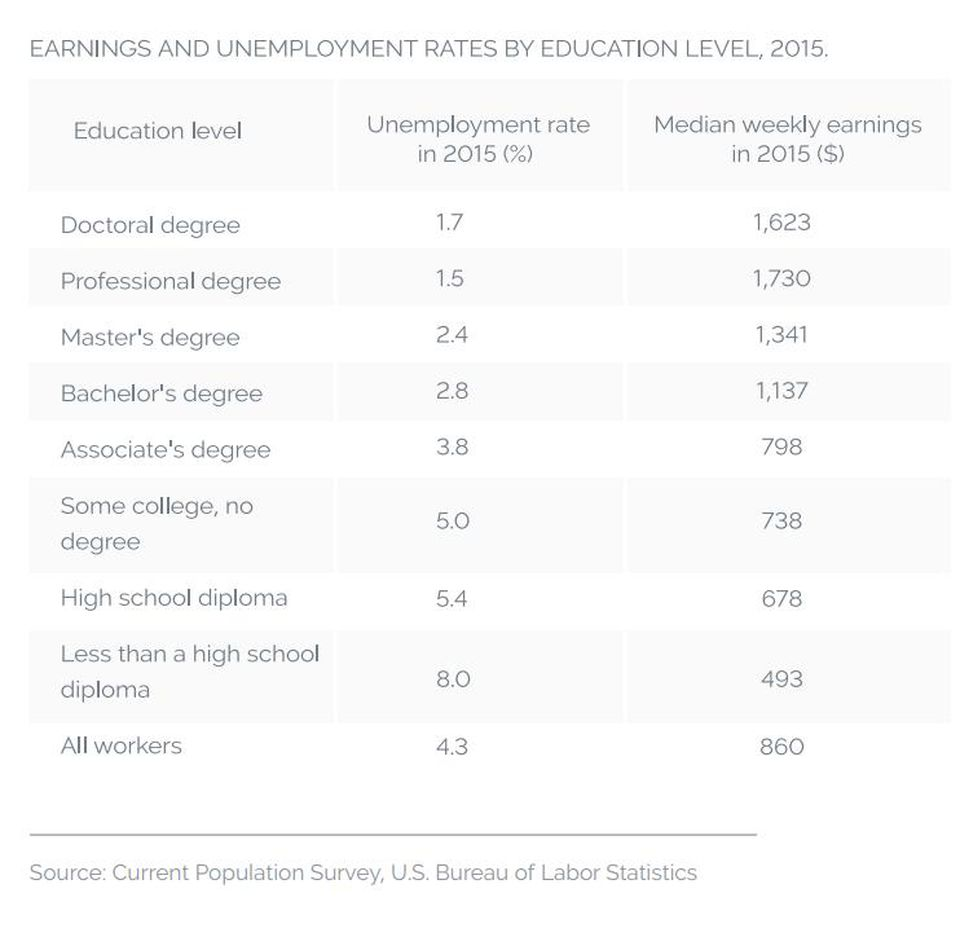
\includegraphics[width=10cm]{./Imagenes/ejemplo2}
	\end{center}

\subsection{¿Cómo lo haces?}	

Primero, debe decidir qué datos son los más importantes. Las estadísticas pueden ser abrumadoras de analizar si no clasifica la información innecesaria. Una vez que decida qué es lo más importante para resaltar, entonces puede transformarlo en una visualización.\\
\\
Sin embargo, para conocer a su público, primero debe saber cómo leer sus datos y cómo usarlos. ¿Qué pregunta intentas responder o problema que intentas resolver?\\

\subsection{Donde empezar}	

El mejor lugar para comenzar sería recopilar sus datos. Esto significa sus datos primero, segundo y tercero . Después de tener todos sus datos en un solo lugar, como una plataforma de gestión de datos (DMP) , puede decidir qué información desea obtener de su historia.\\

La presentación de estos conocimientos a través de la visualización de datos puede mejorar el impacto y las decisiones procesables de la organización.\\

\subsection{Ejemplos de Empresas}	

\begin{itemize}
		\item Airbnb

Storytelling está en el corazón del marketing de Airbnb.Sus centros de mensajería se centran en la comunidad y la hospitalidad local, aprovechando los deseos de los turistas para obtener más experiencias de viaje locales. \\

Solo un ejemplo de cómo la marca utiliza los datos para contar historias atractivas, las historias de AirBnB resuenan constantemente con su público al darles vida a las cosas que les interesan: viajar y nuevas experiencias.\\

		\item Spotify

Spotify recopila datos continuos sobre qué canciones, listas de reproducción y artistas seleccionan sus 30 millones de usuarios.\\  

El servicio de transmisión de música combina esta información con los datos de ubicación y los datos demográficos de los oyentes, y la utiliza para crear contenido original para su blog Spotify Insights.\\

El uso de los datos internos de esta manera ayuda a las marcas como Spotify a crear historias originales basadas en ideas a las que solo ellos pueden acceder, lo que les ayuda a diferenciarse de sus competidores.\\

		\item Google

Los videos de "Año en la búsqueda" de Google se publican anualmente, utilizando sus datos para comunicar los términos más buscados, ofreciendo una perspectiva de "estado de la nación".\\

Google logra evocar una gran variedad de emociones de los espectadores, aprovechando los eventos que han tocado a todos de alguna manera, utilizando datos para identificar exactamente qué temas y eventos atraerán a su audiencia.\\

\end{itemize}

\section{Analisis}
	\label{S:1}


\begin{itemize}

\item Para poder llevar a cabo la implementación del Data Storytelling, es necesario contar con algunas herramientas de tecnologías de la información, tales como: base de datos que nos permitirá comprender el comportamiento y contextos de los grupos a los que queremos dirigirnos, buscaremos datos que nos permitan generar un insight en común, esta base de datos se puede enriquecer, a través de encuestas o formularios brindados por los grupos de interés, es indispensable contar con computadoras y tablets que apoyen la elaboración del contenido a presentar.\\

\item Data Storytelling empleado de manera correcta, mejorará la comunicación entre grupos dentro de una organización, ya que se logrará transmitir las metas y objetivos claros; pero adicionalmente, es importante contar con las personas con las habilidades de comunicación indicadas y poder interpretar los datos encontrados.\\

\item Se pueden emplear las diferentes redes sociales para difundir las historias con los respectivos mensajes que queremos hacer llegar a nuestros grupos objetivos, es por esto que también es necesario poder conocer los máximos beneficios que éstas pueden ofrecer, ya que de nada serviría enviar los mensajes a personas que no formen parte del grupo al que queremos llega.r\\

\item La práctica de storytelling además de aumentar la conversión de ventas crea compromiso, fidelización y flujo, alimentando así aún más un proceso de BIG DATA. Piensa en Netflix. Cuanto más tu ves, más él mejora y más tu quieres ver. Es un ciclo virtuoso en favor de la marca y de los productos y servicios.\\

\end{itemize}

\newpage

%%
	%% Start line numbering here if you want
	%%
	%\linenumbers
	
	%% main text
\section{Conclusion}

		El mundo y la informática en particular, está en constante evolución y estos cambios afectan a muchos ámbitos de nuestra sociedad que exigen un constante esfuerzo de adaptación.\\

La estadística institucional no escapa a esta necesidad y busca nuevas formas de conectar con el público. El Storytelling es una de las nuevas herramientas que pueden favoreceresta adaptación.\\

Usar la data con efectividad requiere ser selectivo y aterrizar información en el contexto de la narrativa que estás comunicando para amplificar la conversación sobre una marca que está teniendo lugar en los medios. Todos estos datos tienen que contar una historia, si no no tienen chiste. \\

Sabemos que la Tecnología de la Información y la analítica, avanzaron rápidamente en sólo unos años. Los modelos de negocio basados en Business Intelligence, usan herramientas flexibles, adaptables al usuario, pensadas para ser eficaces y completas en la visualización de datos.\\

%%
	%% Start line numbering here if you want
	%%
	%\linenumbers
	
	%% main text

	
	
	\newpage
	
	\bibliographystyle{apalike} 	%ESTILO
	\bibliography{BIBLIOGRAFIA}		%ARCHIVO .bib
	
	%% The Appendices part is started with the command \appendix;
	%% appendix sections are then done as normal sections
	%% \appendix
	
	%% \section{}
	%% \label{}
	
	%% References
	%%
	%% Following citation commands can be used in the body text:
	%% Usage of \cite is as follows:
	%%   \cite{key}          ==>>  [#]
	%%   \cite[chap. 2]{key} ==>>  [#, chap. 2]
	%%   \citet{key}         ==>>  Author [#]
	
	%% References with bibTeX database:
	
	
	%% Authors are advised to submit their bibtex database files. They are
	%% requested to list a bibtex style file in the manuscript if they do
	%% not want to use model1-num-names.bst.
	
	%% References without bibTeX database:
	
	% \begin{thebibliography}{00}
	
	%% \bibitem must have the following form:
	%%   \bibitem{key}...
	%%
	
	% \bibitem{}
	
	% \end{thebibliography}
	
	
\end{document}

%%
%% End of file `elsarticle-template-1-num.tex'.
